\documentclass{beamer}
\usetheme[numbering=progressbar]{focus}
\usepackage{tikz}
\usetikzlibrary{positioning}
\usetikzlibrary{shapes,arrows}
\usepackage{transparent}
\usepackage{fancyvrb}
\usepackage{listings}
\definecolor{main}{RGB}{47, 161, 219}
%\definecolor{textcolor}{RGB}{128, 128, 128}
\definecolor{background}{RGB}{240, 247, 255}
\definecolor{textcolor}{RGB}{85, 87, 83}
\title{Passive SSH, a Fast-Lookup Database of SSH Key Materials to Support Incident Response}
\subtitle{}
\author{Alexandre Dulaunoy - Aurelien Thirion}
\titlegraphic{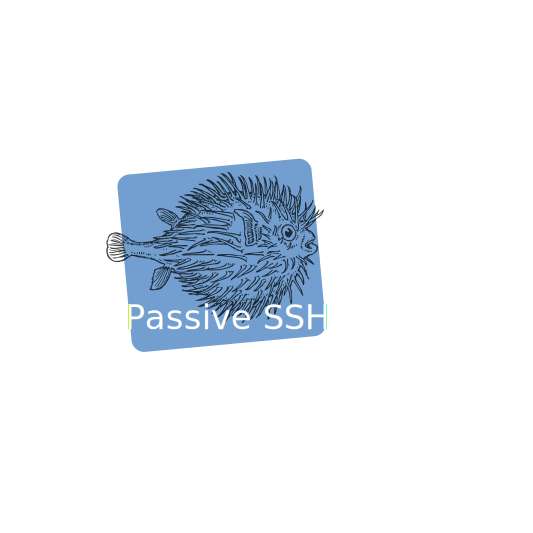
\includegraphics[scale=0.6]{passivessh.pdf}}
\institute{Team CIRCL \\ \url{https://www.d4-project.org/}}
\date{2020-11-16}

\begin{document}
    \begin{frame}
        \maketitle
    \end{frame}

\begin{frame}
        \frametitle{Problem statement}
        \begin{itemize}
                \item CIRCL (and other CSIRTs) have their own passive DNS\footnote{\url{https://www.circl.lu/services/passive-dns/}} and passive SSL{\footnote{\url{https://www.circl.lu/services/passive-ssl/}}} database
                \item Historical data is a companion to incident response, infrastructure attribution and threat intelligence at large
                \item {\bf SSH is a major protocol for remote management} (for normal users but also attackers)
                \item SSH protocol provides a significant {\bf number of fingerprints} to track similar infrastructures (e.g. from banners to key fingerprints)
        \end{itemize}
\end{frame}

\begin{frame}
        \frametitle{Passive SSH design}
        \begin{itemize}
                \item A fast-lookup database to find SSH key per IP, fingerprint or hassh\footnote{\url{https://github.com/salesforce/hassh}}
                \item Supporting the storage of the key materials, key types and banners
                \item {\bf Lightweight design} and supporting different kind of importers (scanner, network capture)
                \item The system can be used externally (for Internet-wide scan) or internally (for internal network ssh infrastructure scanning)
                \item Supporting IPv4, IPv6 but also Tor onion addresses or random TCP ports
        \end{itemize}
\end{frame}

\begin{frame}
        \frametitle{Passive SSH open source software}
        \begin{itemize}
                \item Software written in Python 3 and released as an open source project\footnote{\url{https://github.com/D4-project/passive-ssh}}
                \item The database is a {\bf Redis-compatible backend} (you can use Redis, kv-rocks or any compatible Redis backend)
                \item A sample SSH scanner is included to scan small networks or internal infrastructure
                \item CIRCL provides a {\bf database from an Internet-wide scan} (access can be requested for FIRST, TF-CSIRT and CNW memmbers)
        \end{itemize}
\end{frame}


\begin{frame}
        \frametitle{What's next?}
        \begin{itemize}
               \item A MISP module to get Passive {\bf SSH expansion and pivots in MISP project}
               \item Pcap feeder to Passive SSH
               \item Review of cryptographic materials\footnote{\url{https://github.com/D4-project/snake-oil-crypto}} from existing Passive SSH database
               \item Improvement of the Passive SSH code base and release of version 1.0
        \end{itemize}
\end{frame}

\begin{frame}
\frametitle{Contact}
\begin{itemize}
        \item Get in touch if you want to get access to the {\bf Passive SSH database} (you need to be a FIRST.org, TF-CSIRT or CNW member)
\item Contact: info@circl.lu
\item Source code: \url{https://github.com/D4-project/passive-ssh} -  \url{https://twitter.com/d4_project}
\end{itemize}
\end{frame}


\end{document}
